\documentclass[12pt,a4paper]{report}

\usepackage{geometry}
\usepackage{graphicx}
\usepackage{longtable}
%\usepackage{pgfgantt}
\usepackage[dutch]{babel}
\usepackage{url}
%\usepackage{pgf,pgfplots}
%\usetikzlibrary{fit,calc}
%\usepgfplotslibrary{external}

\geometry{a4paper}

\newcommand{\boxplot}[6]{%
	%#1: center, #2: median, #3: 1/4 quartile, #4: 3/4 quartile, #5: min, #6: max
	\filldraw[fill=white,line width=0.2mm] let \n{boxxl}={#1-0.1}, \n{boxxr}={#1+0.1} in (axis cs:\n{boxxl},#3) rectangle (axis cs:\n{boxxr},#4);   % draw the box
	\draw[line width=0.2mm, color=red] let \n{boxxl}={#1-0.1}, \n{boxxr}={#1+0.1} in (axis cs:\n{boxxl},#2) -- (axis cs:\n{boxxr},#2);             	% median
	\draw[line width=0.2mm] (axis cs:#1,#4) -- (axis cs:#1,#6);                                                                           							% bar up
	\draw[line width=0.2mm] let \n{whiskerl}={#1-0.025}, \n{whiskerr}={#1+0.025} in (axis cs:\n{whiskerl},#6) -- (axis cs:\n{whiskerr},#6);        % upper quartile
	\draw[line width=0.2mm] (axis cs:#1,#3) -- (axis cs:#1,#5);                                                                           							% bar down
	\draw[line width=0.2mm] let \n{whiskerl}={#1-0.025}, \n{whiskerr}={#1+0.025} in (axis cs:\n{whiskerl},#5) -- (axis cs:\n{whiskerr},#5);        % lower quartile
}

\begin{document}

%  Titelblad

\begin{titlepage}

\fontsize{12pt}{14pt}\selectfont

\begin{center}

\vspace{1cm}

\fontsize{14pt}{17pt}\selectfont
% De Faculteit:
\textsc{P\&O Computerwetenschappen - Verslag \\Team Platinum}
\fontsize{12pt}{14pt}\selectfont
\vspace{0.3cm}

\vspace{1.2cm}

%Het academiejaar: aanpassen!
Academiejaar 2011--2012

\vspace{2.8cm}

\fontsize{17.28pt}{21pt}\selectfont

% De titel van de thesis:
{\textsc{Pac-Man in de echte wereld,\\ met behulp van Lego Mindstorms}}

\fontseries{m}
\fontsize{12pt}{14pt}\selectfont

\vspace{2cm}

\includegraphics[height=10cm]{resources/Logo-Kul}

\end{center}
\end{titlepage}

\thispagestyle{empty}

\tableofcontents

\begin{abstract}
Tijdens de uitwerking van dit jaar-overschrijdend groepswerk, bouwen wij een autonome robot met behulp van Lego Mindstorms. Voor de programmatie wordt beroep gedaan op Lejos, een Open Bron project dat een minimale JAVA virtuele machine heeft gemaakt die de plaats kan innemen van de standaard programmatie omgeving van Lego.

Naast de doelstelling om kennis te maken met het ontwikkelen van een autonome robot, willen we in dit project ook ervaring opdoen i.v.m. het werken in teamverband aan een middelgroot softwareproject. Hierbij zijn organisatie van werk, planning, analyse, architectuur,... belangrijke begrippen.

In het tweede semester wordt hier nog eens de nood tot samenwerking met de andere teams aan toegevoegd. Het traject van de autonome robot blijft behouden, maar de verschillende robots zullen nu moeten samenwerken om een gemeenschappelijk doel te bereiken. Om deze samenwerking in goede banen te leiden werd een scheidsrechtercommissie in het leven geroepen om beslissingen te nemen die voor alle teams van belang zijn. Het doel van dit semester is het insluiten van een ``Pac-Man''-robot bestuurd door het didactisch team met behulp van vier autonome ``ghosts''.

In het eerste semester werkten we reeds in een parallel traject aan een simulatieomgeving. Aan de hand van deze omgeving waren we in staat om met meerdere teamleden in parallel software voor de robot te ontwikkelen en te testen zonder nood aan een effectieve fysieke robot. Nu is het ontwikkelen van deze simulator deel geworden van de opdracht en dienen we dus de nodige aanpassingen te doen om het Pac-Man-spel in de computer te simuleren. Het gebruik van een simulator is evident, aangezien we niet kunnen verwachten alle fysieke testen uit te voeren met de 4 teams tegelijk.
\end{abstract}

\chapter{Inleiding}

Het project wordt zoals in het eerste semester begeleid door het gebruik van tussentijdse demo's. Het doel is om zo optimaal mogelijk samen te werken met vier teams om de Pac-Man in te sluiten, hoewel we te allen tijden autonoom beslissingen nemen.

Het doel van de eerste demo is een vereenvoudigde vorm van het einddoel waarbij we een stilstaande Pac-Man zoeken binnen het doolhof. De simulator dient  reeds beschikbaar te zijn en moet drie virtuele robots de fysieke laten bijstaan. Voor de tweede demo mag de commissie beslissen welke doelstellingen passen in het verdere proces richting het einddoel.

Tijdens het eerste semester zijn we er in geslaagd om zeer herbruikbare code te produceren: de architecturale concepten, zoals Robot, Navigator en Model, zijn duidelijk binnen het team en de verdere uitwerking van deze concepten in het tweede semester werd ervaren als een natuurlijke evolutie. Aangezien we te maken hebben met een grote diversiteit aan kleine taken, gebeurt het grootste deel van de taakverdeling week op week.

Het verslag is anders opgebouwd ten opzichte van het vorige semester: er werd gekozen voor een onderverdeling in subsecties per demo binnen een context van hoofdstukken. De opbouw van deze hoofdstukken is erg gelijkend hoewel natuurlijk de inhoud veranderd is t.o.v. het eerste semester. Nieuw zijn de stukken over de strategie i.v.m. de opgegeven spelomgeving, over de samenwerking en over de finale analyse van het jaarproject.

\chapter{Probleemstelling}

De doelstellingen van de demo's worden hier achtereenvolgens beschreven. Zij volgen stapsgewijs een ontwerpproces dat tracht een autonome robot op te leveren die, samen met drie andere ``ghosts'', probeert de Pac-Man in te sluiten.

\section{Demo 1}

Het probleem dat we eerst aanpakken is het zo effici\"ent mogelijk in kaart brengen van een onbekende omgeving met behulp van de vier ``ghosts''. Belangrijk hierbij is natuurlijk dat de gedetecteerde wereld overeenkomt met de realiteit. Tijdens de demo gebruiken we een zgn. hybride simulator: onze eigen robot bestaat in de fysieke wereld, de andere drie zijn virtueel en worden vertegenwoordigd door drie virtuele ``ghosts'' die in de simulator ``leven''.

De ``ghosts'' hebben geen enkele informatie over het doolhof waarin ze zich bevinden, ze kennen wel hun eigen globale positie, maar dan weer niet hun ori\"entatie. Verder staat de Pac-Man stil in het parcours en dient hij enkel gevonden te worden. We dienen ook aan te tonen dat het door de commissie afgesproken communicatieprotocol ge\"implementeerd is.

Elk team wordt tijdens de demo afzonderlijk beoordeeld.
 
\section{Demo 2}
 
De doelstellingen voor demo 2 werden vastgelegd met de resultaten van de eerste demo in het achterhoofd. Deze waren voor sommige teams niet zo goed. Om de kern van de opdracht niet op de lange baan te schuiven wordt in demo 2 toch getracht een stap in de goede richting te nemen. Om de doelstellingen voor demo 2 haalbaar te houden, werd beslist om de Pac-Man nog steeds stil te laten staan. De tweede demo draait daarom volledig rond het samenwerken met de andere teams. Dit is duidelijk een van de essenti\"ele aspecten voor de uiteindelijke demo dat niet uit het oog mag verloren worden.

We volgen de raad op om op voorhand samen te zitten met de andere drie groepen. Het behalen van de doelstellingen is een inspanning van de vier teams samen. Om onverwachte resultaten te voorkomen is samen testen dan ook een noodzaak.

Het doel van deze demo ligt dus in het samen verkennen van het doolhof en het samen insluiten van een stilstaande Pac-Man. We doen dit zowel met de virtuele versie van de simulator als met de gedistribueerde. Initieel krijgt ook elk team de kans om eerst nogmaals zijn hybride simulator te tonen en de vooruitgang ten opzichte van de eerste demo aan te duiden.

\section{Demo 3}

\subsection{Verkenning}

De robots rijden in een onbekend doolhof. Alle info die verzameld wordt door de vier ghosts draagt bij tot het cre\"eren van een individuele map die mogelijk inconsistenties bevat. Alle juiste info over het doolhof zal direct bijdragen tot het hoofddoel, namelijk het vangen van de Pac-Man. Elke robot communiceert zijn gevonden informatie en probeert zo veel mogelijk informatie te verzamelen over de voor hem onbekende wereld. Elke fout van \'e\'en van de robots kan reeds fataal zijn voor het kunnen opbouwen van een beeld van de omgeving. We proberen dus een zo robuust mogelijke robot te maken die zo effici\"ent mogelijk zijn eigen info verzamelt en met de nodige voorzichtigheid andere informatie hierin verwerkt.

\subsection{Pac-Man}

Het Pac-Man spel zelf kunnen we winnen door alle vluchtwegen van de Pac-Man af te sluiten. Dit houdt in dat alle omliggende sectoren door een ``ghost'' bezet of door een muur afgeschermd worden. Men wint enkel als alle robots die meewerken aan de insluiting ook effectief aangeven dat ze gewonnen hebben via hun grafische interface. De probleemstelling vereist dus een afdoende samenwerking, waarbij een consensus moet bereikt worden over de verzamelde informatie en de te volgen strategie.

\chapter{Scheidsrechtercommissie}

Deze commissie staat in voor het nemen van beslissingen die betrekking hebben op afspraken tussen de verschillende teams en het didactische team. Hierbij kunnen we deze beslissingen groeperen in:

\begin{itemize}
	\item De verdere regels waarmee de spelomgeving beperkt wordt.
	\item Afspraken die noodzakelijk zijn voor de samenwerking van de teams.
\end{itemize}

\section{Spelregels}

\subsection{Spelwereld}

De spelwereld bestaat uit aangepaste panelen uit het eerste semester. Er is een raster van witte lijnen ge\"introduceerd waar muren kunnen staan. Dit komt neer op een mogelijke herschaling van de panelen met een factor vier. Deze nieuwe minimumeenheid aan oppervlakte noemen we sectoren. Deze sectoren zijn belangrijk voor de plaatsbepaling. Het doolhof is volledig ommuurd en de absolute afmetingen worden op voorhand opgegeven.

\subsection{Pac-Man}

De Pac-Man wordt zichtbaar gemaakt door een infrarood-beacon dat kan opgemerkt worden met behulp van de voorziene IR-sensor. Het didactisch team kiest waar deze vertrekt en bestuurt hem tijdens de demo's. Hij mag enkel bewegen op sectoren waar zich geen ``ghosts'' bevinden.

De beweging van Pac-Man is beperkt tot het rechtdoor oversteken van de witte lijnen die de sectoren scheiden.

Insluiting van Pac-Man is gedefinieerd als het niet meer kunnen bewegen van de Pac-Man of het ingesloten zijn in een doodlopend pad.

\subsection{Ghosts}

De ghosts vertrekken op de vier hoekpunten van het doolhof, zodat de verkenning van het doolhof zo snel mogelijk van start kan gaan. De ori\"entatie van de robot is onbekend hoewel de hoek t.o.v. het assenstelsel wel een veelvoud is van 90 graden.


\section{Communicatieprotocol}

We verwijzen naar de offici\"ele documentatie van het Ghost Protocol. Ten tijde van het schrijven van dit verslag was versie 1.0 beschikbaar. Het Ghost Protocol is het resultaat van een werkgroep die aangesteld werd door de scheidsrechtercommissie. In dit deel van het verslag belichten we de positieve en de negatieve punten van het voorgestelde protocol en bespreken de voor- en nadelen ervan mbt. onze eigen ontwikkeling.

\subsection{Voordelen}

Het collaborative diffusion algoritme waarop onze implementatie gebaseerd is, heeft zeer weinig informatie nodig van de andere robots. Het algoritme werkt zelfs met enkel omgeving-gerelateerde informatie en de positie van de andere robots in het doolhof. De minimale subset van commando's die in het protocol moeten aanwezig zijn voor onze implementatie zijn:

\begin{itemize}
	\item{ [naam] position [p:coord]}
	\item{ [naam] discover [p:coord] [w:int]}
	\item{ [naam] pacman [p:coord] [a:angle]}
	\item{ [naam] barcode [p:coord] }
	\item{ [naam] captured }
\end{itemize}

Deze functionaliteit is aanwezig in het huidige protocol, dus is het compatibel met onze verkozen implementatie.

\subsection{Nadelen}

In het algemeen ondervinden we geen nadelen van de beslissingen die genomen zijn. Aangezien we voldoende informatie kunnen verzamelen met een subset, zal het volledige protocol slechts een marginale implementatie-meerkost met zich meebrengen. Volgens ons kan het protocol wel sterk vereenvoudigd worden. Aangezien die slechts vervelend is en niet als nadeel beschouwd kan worden, voegen we onze opmerkingen toe in de vorm van een analyse.

\subsection{Analyse van het GhostProtocol}

De ``join'' procedure lijkt overbodig. Wanneer een spook laattijdig ``joint'', zal hij gewoon de volgende berichten horen en zijn wereldbeeld beginnen opbouwen. Eventueel kan een commando toegevoegd worden om reeds gestuurde informatie opnieuw te sturen. In een latere versie van het protocol werd het ``showmap'' commando toegevoegd, wat deze functie gedeeltelijk vervult. Dit overlapt gedeeltelijk met het ``join'' principe. Bovendien eist de procedure dat er exact 4 spoken zijn. Indien een spook uitvalt, of een extra spook op het kanaal komt, zorgt dit voor problemen. Hiervoor werd een 'override' commando toegevoegd, om toch te starten indien er een spook geen join stuurt. De protocolrestrictie voor 4 spoken is volgens ons volledig onnodig, net als de join procedure. 

In plaats van dynamisch namen uit te wisselen kunnen evengoed vaste namen afgesproken worden, dit zou het protocol eenvoudiger maken. Er zijn tal van mogelijkheden: alle teams hebben een naam of de echte namen van de vier spoken kunnen gehanteerd worden. Een conventie lijkt ons hier ver boven een configuratie te verkiezen.

Voor het ``discover'' commando lijkt het beter om een bitfield te gebruiken voor de aanduiding van de muren. Omdat er zeer veel discover commando's gestuurd kunnen worden, kan dit de overhead op de communicatie verkleinen en zelfs het parsen vereenvoudigen. Met eenvoudige bit-wise shift operaties kan getest worden of een tegel een muur heeft of niet. Dit geldt tevens ook voor de commando's zelf. Ook deze waren beter vervangen door getallen, zodat alle informatie louter numeriek was en optimaler verstuurd zou kunnen worden.

Het ``plan'' commando is naar onze mening onvolledig. Het doorsturen van een pad is pas nuttig indien er ook een ``election''-procedure voorzien zou zijn. Verder is zonder een tijdsynchronisatie en informatie over hoe snel de robot zijn pad aflegt al deze informatie nutteloos.

Voor ons algoritme is dit commando tevens volledig overbodig. Onze robot rijdt op enkel informatie van het doolhof, de positie van de andere robots en Pac-Man. De pad informatie zal initieel niet gebruikt worden in onze implementatie.

Nog een algemene opmerking is dat het protocol moeilijk te parsen is door combinatie van strings en numerieke waardes, inconsistenties in de structuur van de commando's, gebruik van verschillende soorten scheidingstekens, enz.

Oorspronkelijk was het idee dat het Ghost Protocol letterlijk gebruikt zou worden in het Maze Protocol - het Maze Protocol is een doorslag van het Ghost Protocol en wordt gebruikt om doolhoven te beschrijven, bvb. voor de simulator. Op deze manier zou de implementatie van het Ghost Protocol kunnen hergebruikt worden. Spijtig genoeg zijn er enkele aanpassingen doorgevoerd waardoor het nu niet meer 100\% compatibel is met het Ghost Protocol. Deze aanpassingen waren naar onze mening beter doorgevoerd geweest op het Ghost Protocol zelf.

\subsection{Aanpassingen Demo 2}

Het ``barcode'' commando wordt vervangen door een ``barcodeat'' commando, dit is een vooruitgang aangezien er nu geen logica meer voorzien moet worden om de barcodes aan een positie te linken. 

Er werd eveneens een ``removebarcode'' toegevoegd om teams toe te laten eerdere transmissies omtrent barcodes ongedaan te maken.


\chapter{Robot}

\section{Demo 1}

\subsection{Fysiek ontwerp}

Door de gewijzigde specificaties van de fysieke omgeving en de extra infrarood sensor, moesten enkele wijzigingen gemaakt worden aan de fysieke robot. Zo zijn de druksensoren verwijderd om een sensorpoort vrij te maken voor de infraroodsensor. Bovendien is het in dit project noodzakelijk om zo precies mogelijk door het midden van de sectoren te rijden - touch-sensoren zijn minder van toepassing in deze strategie. Aangezien het doolhof minder breed is (sectoren zijn 40 centimeter in plaats van 80) zijn de extra wielen weggehaald om het geheel iets slanker te maken.

Verder is ook de motor, die de sonar laat draaien, iets naar onder en naar het midden verplaatst. Hierdoor hebben we de tandwielen tussen de motor en de sensor kunnen elimineren waardoor de sensor rechtstreeks op de motor zit. Om eenvoudiger de uitvoer op het scherm van de robot te kunnen lezen, is de ``NXT Brick'' omgedraaid, zodat het scherm zich nu aan de onderzijde van de robot bevindt. Hiermee kunnen we de robot gemakkelijker besturen en connecteren met de computer.

\subsection{IR-sensor}

De infraroodsensor werd vooraan in het midden van de robot aangebracht, net boven de lichtsensor. Het uitlezen van deze sensor zorgde voor een aantal problemen. De maximale gemeten afstand kwam niet overeen met de specificatie van de IR-bal en sensor. Het bleek dat de Lejos implementatie verouderd was en niet alle mogelijkheden van de sensor ondersteunde. Met behulp van de broncode van Lejos versie 9.0 en enkele aanpassingen, is ons team er in geslaagd de verschillende modi van de sensor te activeren.

Uit testen bleek dat er voor de bal verschillende AC modi en \'e\'en DC modus is. De sensor heeft \'e\'en AC modus en \'e\'en DC modus. De AC modus van de bal die speciaal voor de sensor ontwikkeld was, werkte uiteindelijk het beste. De sensor had dan een reikwijdte van 5 meter in tegenstelling tot ongeveer 80 cm bij andere modi.

In figuur \ref{fig:plotIR} kan men zien dat de gemeten lichtsterkte exponentieel afneemt ten opzichte van de afstand tot de lichtbron.
Hieruit zou men een schatting kunnen maken van de afstand tot de bron. In grafiek \ref{fig:boxplotIR} kan men de variatie van de IR-sensor zien voor verschillende afstanden. We zien dat de varianties zeer klein zijn in vergelijking met de lichtsterkte. Een afstandsschatting lijkt dus goed mogelijk.

\begin{figure}[htbp]
  \centering
  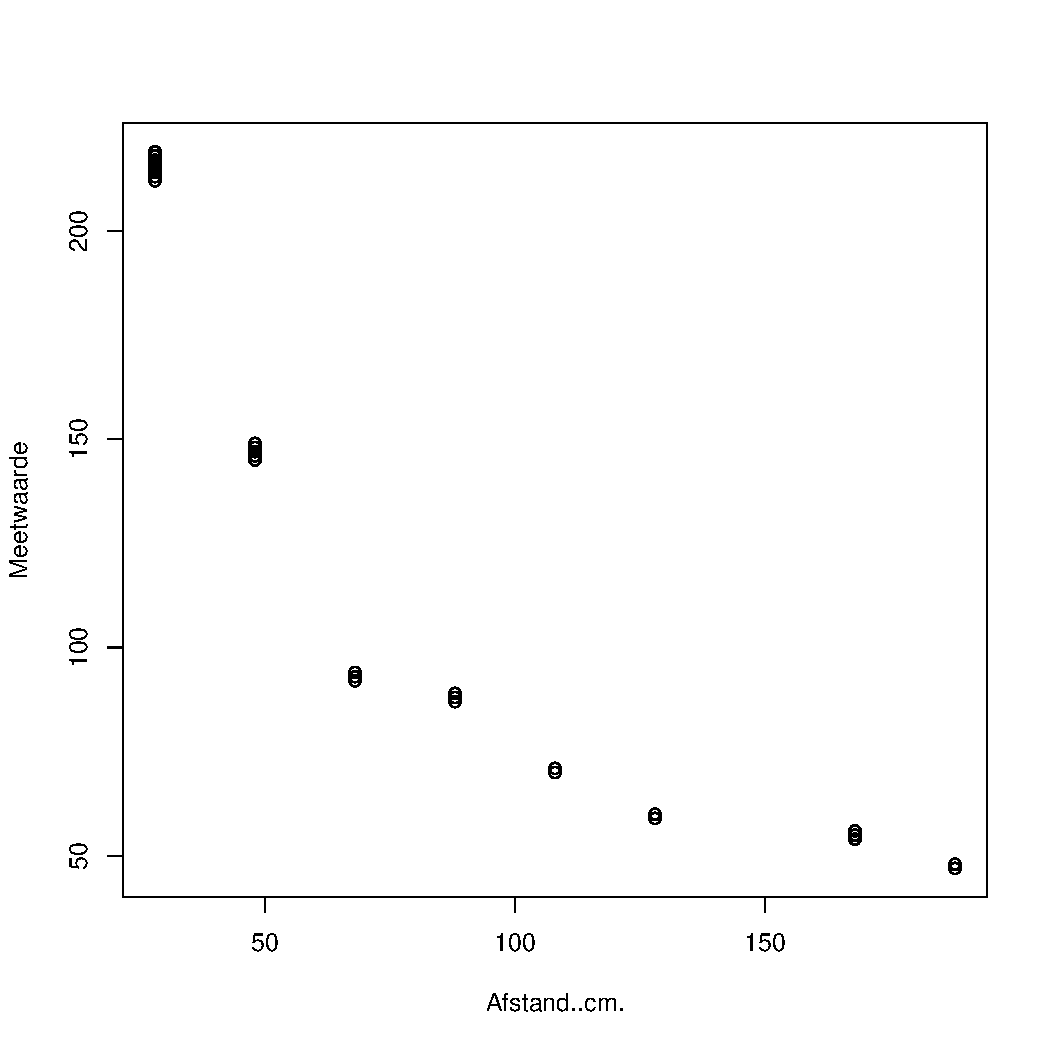
\includegraphics[width=85mm]{resources/plotIR.pdf}
  \caption{De meetwaarden van de IR-sensor volgens een bepaalde afstand}
  \label{fig:plotIR}
\end{figure}

\begin{figure}
\begin{center}
 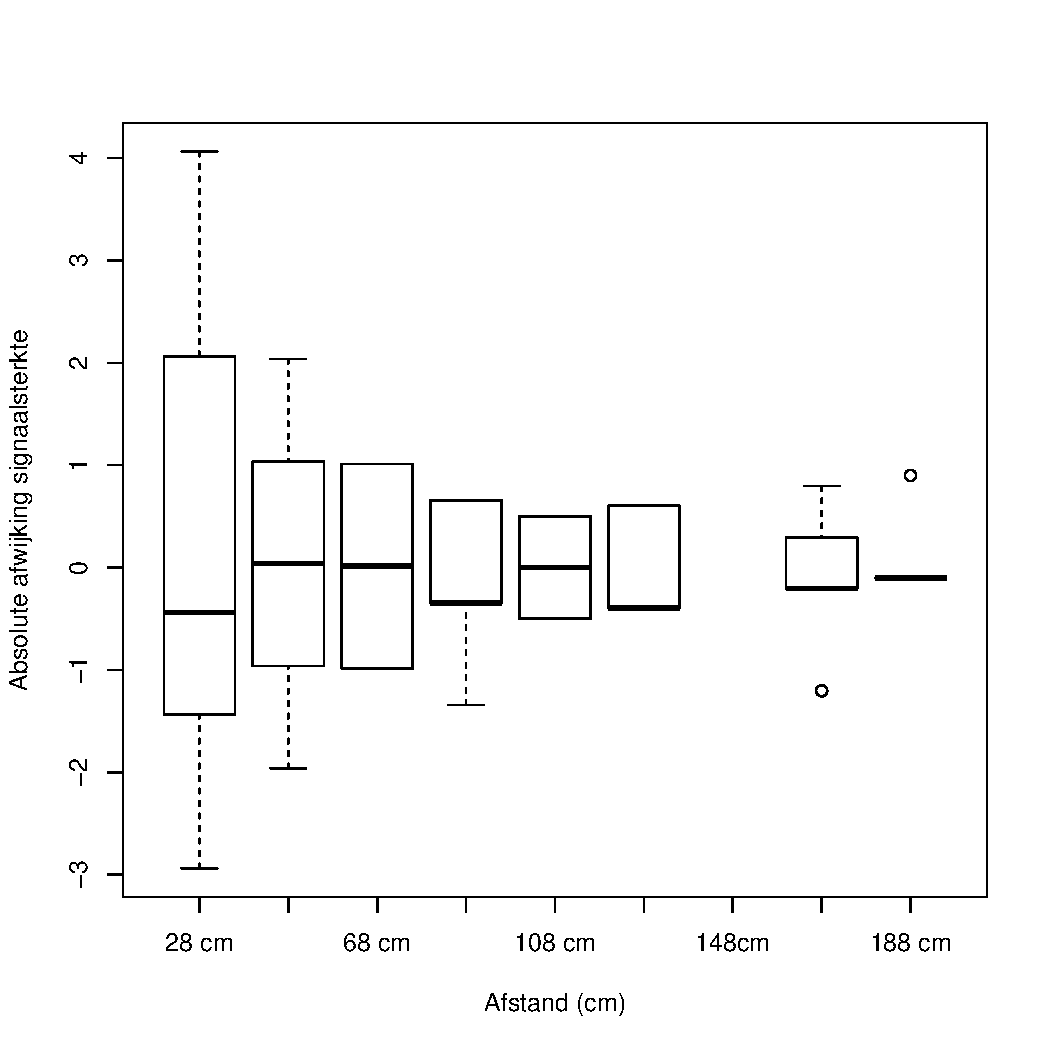
\includegraphics[width=85mm]{./resources/bloxplotIR.pdf}
 \caption{Sensorwaarden van de IR-sensor bij verschillende afstanden}
 \label{fig:boxplotIR}
\end{center}
\end{figure}

Uit testen blijkt dat een significante hoeveelheid van het IR licht via weerkaatsingen door de infraroodsensor gedetecteerd wordt.
De sterkte is bij weerkaatsing herkenbaar lager dan bij een rechtstreekse detectie (zie grafiek \ref{fig:boxplotSpiegeling}).  Men kan dus eventueel ook aan de hand van de signaalsterkte herkennen of de Pac-Man zich bvb. achter een hoek bevindt. In dit geval kan deze meting zelfs best genegeerd worden. Het reconstrueren van een weerkaatsingpatroon is een zeer moeilijke opgave.

\begin{figure}
\begin{center}
 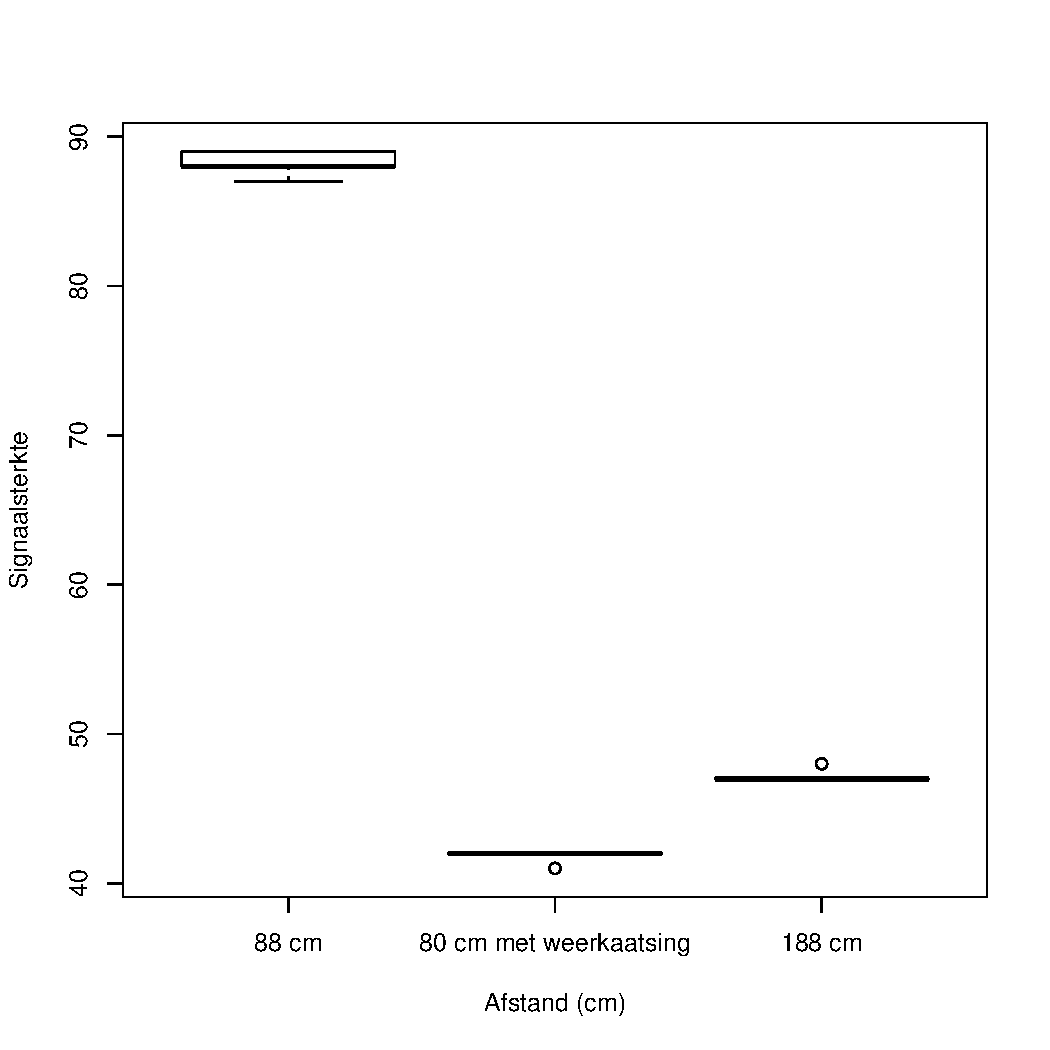
\includegraphics[width=85mm]{./resources/boxplotSpiegeling.pdf}
 \caption{Sensorwaarden van de IR-sensor bij weerkaatsing en verschillende afstanden}
 \label{fig:boxplotSpiegeling}
\end{center}
\end{figure}

Een nadeel van zo'n filtering is dat deze de afstand waarop geschat kan worden inperkt. Zoals men kan zien op de grafiek \ref{fig:boxplotSpiegeling}, kunnen we geen afstanden van meer dan 160 cm (4 sectoren) onderscheiden van weerkaatsingen. Voor demo 2 en 3 zal moeten afgewogen worden wat de beste oplossing is: een grotere gemeten afstand maar misschien niet nauwkeurig, of een grotere zekerheid garanderen. Hier zal ook rekening gehouden moeten worden met de andere teams. 

\section{Demo 2}

Aangezien in demo 1 bleek dat de lichtsensor niet goed functioneerde, zullen we naar demo 2 toe de lichtsensor opnieuw van dichterbij bekijken. Het is moeilijk om de exacte condities van de demo na te bootsen, maar we kunnen wel de in de databank opgeslagen gegevens analyseren. Tevens zullen andere pistes bewandeld worden, op zoek naar een stabieler resultaat. Een eerste test zal opnieuw het plaatsten van een ``kapje'' zijn, zoals in het eerste semester getest werd. Deze aanpak werd toen niet gebruikt vanwege de hoogteverschillen in het parcours. 

\section{Demo 3}

Dit deel wordt later toegevoegd.

\chapter{Strategie}

Aangezien wij ons slechts sinds enkele maanden begeven op het terrein van autonome robots en artifici\"ele intelligentie, zou het dom zijn te veronderstellen dat er ons nog niemand is voor gegaan. We hebben daarom een literatuurstudie rond de concepten van Pac-Man en autonome ``ghosts'' gedaan.

We vonden een paper omtrent ``Collaborate Diffusion'' \cite{Repenning06}. Hierin wordt voorgesteld om een vorm van ``Hill Climbing'' toe te passen om zo verschillende autonome ``ghosts'' toe te laten samen te werken om een ``Pac-Man'' te achtervolgen. Hierbij hebben zij geen nood aan bijkomende onderlinge communicatie naast de informatie over de omgeving.

Ondanks het feit dat we geen overeenstemming met de andere teams konden bereiken om allen dit algoritme te implementeren, blijft het een zeer interessant algoritme om toe te passen voor het bepalen van ons eigen pad.

\section{Achtervolgstrategie}

Wanneer de Pac-Man gezien wordt, stuurt deze een ``geur'' uit. Deze plant zich langs gekende sectoren voort. Dit wordt gedaan door het gemiddelde van de 4 omliggende sectoren te berekenen, indien er een muur staat is de waarde 0. Zo ontstaat er een ``hoogte-kaart'' met aan de top een Pac-Man. De ``ghosts'' kunnen nu aan de hand van een eenvoudig ``Hill Climbing'' algoritme een optimale weg volgen naar de Pac-Man.

Wanneer een ``ghost'' de Pac-Man opmerkt, kan deze positie op de kaart een zeer hoge waarde gegeven worden. Deze kaart wordt vaak herberekend en de geur van een Pac-Man zal dus snel verdwijnen. En dit is zoals het in de realiteit ook zal zijn. De Pac-Man beweegt zich doorheen het doolhof en zal niet op \'e\'en plek blijven wachten. Als een Pac-Man meerdere keren gezien wordt, zal zijn positie ook een constantere ``geur'' verspreiden, waardoor de ``ghosts'' van alle kanten op hem kunnen naderen. 

Een handige manier om de geur van een Pac-Man te visualiseren is door middel van een kleurenpallet. We hebben hierbij gekozen voor het kleurenpallet zoals dit in de natuur voorkomt. Figuur \ref{fig:colormap} toont dit kleurenpallet met een aanduiding van de overeenkomstige interne numerieke waarde die aan een sector toegekend wordt om de intensiteit van de ``geur'' voor te stellen.

\begin{figure}[htbp]
  \centering
  \includegraphics[width=150mm]{resources/colormap.png}
  \caption{Kleuren en voorgestelde interne ``geur''-waarden}
  \label{fig:colormap}
\end{figure}

Figuur \ref{fig:hillclimbing1} toont een uitgangssituatie met een Pac-Man die een een uitdijende ``geur'' verspreidt.

\begin{figure}[htbp]
  \centering
  \includegraphics[width=50mm]{resources/hillclimbing1.png}
  \caption{Hill Climbing}
  \label{fig:hillclimbing1}
\end{figure}

Om te voorkomen dat ``ghosts'' allemaal dezelfde weg volgen en enkel achter Pac-Man lopen slorpt iedere ``ghost'' de geur op door de waarde van zijn huidige sector op 0 te zetten. Hierdoor ontstaat er een dal rond iedere ``ghost'' en zullen de anderen een omweg zoeken. Dit zorgt er ook voor dat de ``ghosts'' elkaar van nature uit ontwijken en niet zullen botsen. Figuur \ref{fig:hillclimbing2} illustreert dat, eens een ``ghost'' een bepaalde ``beste'' route naar de Pac-Man heeft ingeslagen, het pad achter hem minder interessant wordt voor de overige achtervolgers. In de voorstelling ontstaat er een ``deuk'' in de ``geur'' achter de ``ghost''. Andere ``ghosts'' zullen daarom eerder andere paden, parallel aan het reeds ingeslagen pad, kiezen.

\begin{figure}[htbp]
  \centering
  \includegraphics[width=50mm]{resources/hillclimbing2.png}
  \caption{Hill Climbing met afsluiting van pad}
  \label{fig:hillclimbing2}
\end{figure}

\section{Verkenstrategie}

De verkenstrategie is gebaseerd op hetzelfde principe. Hier is er niet \'e\'en bron die een geur uitstuurt, maar iedere onbekende sector stuurt een geur uit. De robot zal hierdoor altijd naar het dichtstbijzijnde en het meest onverkende stuk van het doolhof willen gaan. Daarnaast zorgt dit principe er ook voor dat een robot zal terugkeren op zijn stappen en automatisch terugkeert naar achtergelaten onbekende sectoren. We kunnen stellen dat het algoritme impliciet ``Depth-First-Search'' implementeert. Figuur \ref{fig:dfs} toont een robot die een onbekend doolhof aan het verkennen is. De felgroene sectoren zijn onbekende sectoren en hebben een hogere waarde dan de reeds bezochte sectoren.

\begin{figure}[htbp]
  \centering
  \includegraphics[width=50mm]{resources/dfs.png}
  \caption{Hill Climbing met impliciet ``Depth-First-Search'' zoekgedrag}
  \label{fig:dfs}
\end{figure}

Het toepassen van hetzelfde algoritme voor beide deelproblemen, levert ons in essentie een enkelvoudige implementatie van beide. Door het toekennen van goed gekozen waarden aan onbekende sectoren en aan sectoren waar Pac-Man werd gezien, stelt het algoritme ons in staat om steeds het optimale doel te kiezen. Wanneer er zich geen pad bevindt naar de Pac-Man zal een ``ghost'' onbekende sectoren trachten te verkennen. Wanneer er een pad bestaat naar de Pac-Man zal zijn ``geur'' dit pad nog extra versterken en zal een ``ghost'' automatisch hierdoor aangetrokken worden.

\chapter{Softwaredesign}

In het eerste semester hadden we reeds een redelijk uitgebreid raamwerk opgebouwd om robots samen te stellen uit componenten. Dankzij dit werk kunnen we in het tweede semester hier op verder bouwen door de bestaande concepten verder te verfijnen en uit te breiden.

\section{Robot}

Het klasse diagram op figuur \ref{uml:design-semester1} toont de belangrijkste bouwstenen van ons robot-raamwerk, zoals dit tijdens het eerste semester werd ontworpen: een Robot-entiteit beschikt over een RobotAPI om met de fysieke robot informatie uit te wisselen. Deze informatie heeft betrekking op de gemeten waarden van de verschillende sensoren als ook het instellen van de motoren. De RobotAPI stelt ons in staat om door het vervangen van \'e\'en enkele klasse, identiek dezelfde Robot-entiteit te gebruiken in een echte fysieke robot, alsook in een gesimuleerde wereld.

\begin{figure}[htbp]
  \centering
  \includegraphics[width=110mm]{resources/design-semester1.png}
  \caption{Design $1^e$ semester}
  \label{uml:design-semester1}
\end{figure}

De Robot beschikt verder over een Model waarin alle informatie uit de wereld wordt samengebracht. Dit Model kan verrijkt of bijgewerkt worden door zgn. ModelProcessors. Deze onderzoeken bepaalde delen van het Model en trachten hieruit informatie van een hoger niveau te distilleren. Voorbeelden hiervan zijn processors die op basis van metingen door de sonar-sensor bepalen waar er zich muren bevinden.

Tot slot heeft de Robot ook een Navigator die op basis van de informatie in het Model bepaalt waarheen de Robot dient te rijden. De navigator geeft zeer basische instructies aan de Robot, in de vorm van ``beweeg voor- of achterwaarts'' en ``draai zoveel graden''.

Om met de Robot te kunnen communiceren is een RobotAgent voorzien, waarlangs berichten kunnen verzonden en ontvangen worden.

Het is duidelijk dat dit raamwerk een sterk herbruikbare basis biedt om verschillende robots te bouwen. Dit heeft al tijdens het eerste semester zijn nut bewezen, maar komt nog sterker naar voor bij aanvang van het tweede semester. Door het maken van een nieuwe specifieke Navigator en bijhorend Model met Modelprocessors, kunnen we opnieuw een robot samenstellen.

\subsection{Driver}

Ofschoon we een nieuwe Navigator zouden kunnen maken die perfect zou passen, werd snel duidelijk dat er een verfijning van het raamwerk mogelijk was: daar waar tijdens het eerste semester de robot geen resolutie had bij het rijden, is dit in het tweede semester wel het geval. Door het introduceren van het concept van sectoren is er een duidelijk onderscheid tussen het operationele en strategische aspect van het besturen van de robot. Operationeel dient de robot optimaal van sector naar sector te rijden, zodat op strategisch niveau kan geredeneerd worden in termen van deze sectoren.

De functionaliteit om van sector naar sector te rijden zou typisch terecht gekomen zijn in een Navigator-implementatie. Deze wordt in het verfijnde raamwerk ondergebracht in een zgn. ``Driver''. Het klasse diagram op figuur \ref{uml:design-semster2} toont dat de introductie van de Driver letterlijk een uitbreiding is van het bestaande raamwerk. Voor het tweede semester is er tevens een eerste implementatie van de Driver gemaakt in de vorm van een ``ManhattanDriver''\footnote{Zo genoemd naar analogie met Manhattan Distance en de Taxicab geometrie.} 

\begin{figure}[htbp]
  \centering
  \includegraphics[width=110mm]{resources/design-semester2.png}
  \caption{Design $2^e$ semester}
  \label{uml:design-semster2}
\end{figure}

\subsection{Grids en Sectoren}

De Navigator kan zich nu specifiek toeleggen op het bepalen van de volgende Sector, waarheen de Driver moet rijden. Om deze taak te ondersteunen werden de concepten Grid, Sector en Agent in het leven geroepen. Het klasse diagram op figuur \ref{uml:grids-sectoren} geeft een overzicht van hun samenhang en van de effectieve implementaties die samen de zgn. ``GhostRobot'' opbouwen.

\begin{figure}[htbp]
  \centering
  \includegraphics[width=200mm, angle=90]{resources/grids-sectors.png}
  \caption{Design Grids en Sectoren}
  \label{uml:grids-sectoren}
\end{figure}

Centraal staat het concept van de Sector in een Grid. Een Sector heeft een co\"ordinaat relatief t.o.v. de Grid waarop het zich bevindt, heeft potentieel 4 muren, elk al dan niet gekend, heeft een waarde en kan bezet worden door een Agent. De waarde van een Sector zal gebruikt worden om de hoogte of de intensiteit van de geur weer te geven. Een Agent kan zich doorheen de Grid bewegen langs de Sectoren. De meeste functionaliteit van een Agent is ge\"implementeerd in een abstract basis klasse, MovingAgent. Mits kleine configuratie aanpassingen, implementeren de PacmanAgent en GhostAgent zo de agents die op de Grid voorkomen. Een ProxyAgent werd gebruikt om in een simulator een echte Agent voor te stellen die de volledige Grid nog niet kent en de StaticTargetAgent werd speciaal voorzien voor de voorbereiding van de eerste demo.

Optioneel kan aan een Grid ook een GridView gegeven worden. Deze voorziet een visualisatie van de Grid en kan op verschillende manieren ingevuld worden. Voor dit project hebben we twee implementaties gemaakt: enerzijds een ConsoleGridView die gedetailleerde informatie over de Sectoren weergeeft en een SwingGridView die een grafische voorstelling geeft van de Grid. Deze laatste wordt gebruikt voor de visualisatie in o.a. de simulator.

Een Grid beschikt ook over een GridProcessor. Net zoals de ModelProcessor kan dit een geschakelde lijst van Processoren zijn die de Grid kunnen ondervragen en bijwerken. Zo hebben we een DiffusionGridProcessor ge\"implementeerd die de waarde van de Sectoren zal bijwerken volgens het eerder beschreven algoritme.

De nieuwe robot zal ook informatie van andere robots ontvangen. Deze worden allemaal opgeslagen in een zelfde Grid. Een tweede implementatie van het Grid concept, de zgn. AggregatedGrid, is in staat om een aantal verschillende grids samen in beschouwing te nemen en de ``som'' van deze als een geaggregeerd beeld aan te bieden.

\subsection{GhostRobot}

Het klasse diagram op figuur \ref{uml:ghostrobot} geeft tot slot de volledige compositie van de nieuwe ``GhostRobot'' weer. De GhostRobot beschikt over een GhostModel, GhostNavigator en GhostDriver.

\begin{figure}[htbp]
  \centering
  \includegraphics[width=110mm]{resources/ghostrobot.png}
  \caption{Compositie GhostRobot}
  \label{uml:ghostrobot}
\end{figure}

Het GhostModel bevat Grids voor elk van de andere robots alsook een AggregatedGrid voor de eigen Agent. Zolang er geen gemeenschappelijk referentiepunt\footnote{Referentiepunten worden op het parcours voorgesteld door geori\"enteerde barcodes.} is gevonden zijn de verschillende Grids niet met elkaar in verband te brengen. Wanneer er echter een gemeenschappelijk referentiepunt gevonden is, kan de corresponderende Grid van de andere robot toegevoegd worden aan de eigen AggregatedGrid, waardoor de informatie van beide Grids gecombineerd wordt en een ruimer wereldbeeld beschikbaar wordt.

De eigen AggregatedGrid beschikt ook over een DiffusingGridProcessor die het algoritme voor het bepalen van de waarde van een Sector zal toepassen op de AggregatedGrid, waardoor de GhostNavigator een redelijk eenvoudige beslissing kan nemen op basis van de waarden van de vier aangrenzende sectoren.

Het GhostModel is verder voorzien van een aantal ModelProcessoren die de inkomende informatie verwerken tot informatie waarmee de GhostNavigator beslissingen kan nemen. Enerzijds is er een InboxProcessor die de binnenkomende berichten van de andere robots omzet in aanpassingen aan de verschillende Grids in het GhostModel. Anderzijds is er de WallDetectorProcessor die op basis van de gemeten waarden door de sonar-sensor een beeld zal samenstellen van de huidige Sector. Tot slot is er de GridUpdateProcessor die de nieuwe muur-informatie zal verwerken in de eigen Grid en eventueel nieuwe sectoren zal toevoegen.\footnote{Naast deze drie ModelProcessoren zijn er nog andere actief. Het betreft hier bvb. de LineModelProcessor of de WallDetectionModelProcessor. Deze zorgen voor informatie die door de Driver zal gebruikt worden om optimaal naar de volgende sector te rijden. Veel van deze ModelProcessoren maakten reeds deel uit van de robots uit het eerste semester.}

\subsection{Performantie}
\label{sect:performance}

Met de expliciete keuze om alle software op de robot zelf te implementeren, zijn we natuurlijk gebonden aan de beperkingen van de robot. Enerzijds heeft deze geen processor die te vergelijken is met de processors van hedendaagse computers. Dit is echter voor onze architectuur en gekozen zoekstrategie geen probleem. Door gebruik te maken van een zeer eenvoudig ``local hill climbing'' algoritme, gebaseerd op het principe van ``Collaborate Diffusion'', vragen we zeer weinig van de processor. We slagen er in om een ``frame rate'' te bekomen die rond de 80 FPS \footnote{Frames Per Second is een term die uit de grafische sector komt en weergeeft hoeveel beelden per seconde gemaakt worden, maar wordt ook gebruikt in andere contexten. Een ``frame'' is dan het geheel van taken. Voor onze robot bestaat \'e\'en frame uit het opvragen van de sensorwaarden, het bijwerken van het Model, het kiezen van een volgende actie en het initi\"eren van de uitvoering.} ligt, wat betekent dat de frequentie waarmee de robot al zijn taken uitvoert meer dan hoog genoeg is voor de taken die moeten uitgevoerd worden. Proefondervindelijk hebben we vastgesteld dat een frame rate van 60 FPS een minimum is om de verschillende taken naar behoren uit te voeren.

\subsubsection{Geheugengebruik}

Het aspect geheugen is dan weer wel een sterk beperkende factor. De robot beschikt slechts over een werkgeheugen van 64KB waarvan een deel reeds wordt ingenomen door het geladen programma. Tijdens het eerste semester was de hoeveelheid informatie die opgeslagen werd in het Model nagenoeg constant, of had ten minste een gekende bovengrens. In het tweede semester moeten we echter informatie bijhouden over het speelveld waarop we ons bewegen. Aangezien we op voorhand niet weten hoe groot dit speelveld is kunnen we niet op voorhand een bovengrens bepalen voor het geheugen nodig om deze informatie op te slagen. Daarbij komt dat we dit speelveld niet alleen moeten bijhouden voor onze eigen robot, maar ook voor de drie andere robots.

Intern stellen we het speelveld of Map voor als een verzameling sectoren, die verbonden zijn met elkaar door bi-directionele verwijzingen. Telkens een robot een nieuwe sector ``ontdekt'' wordt er intern ook een nieuw Sector object aangemaakt. De grootte van zo'n Sector object is dus bepalend voor de hoeveelheid sectoren we maximaal kunnen bijhouden in het geheugen van de robot.

Vlak voor demo 1, was een Sector ongeveer 370 bytes groot en konden we ongeveer 145 Sectoren opslaan in ons geheugen. In een worst-case scenario betekent dit dat we per robot 36 sectoren konden opslaan, wat overeenkomt met een speelveld van 6 bij 6. We hebben vervolgens twee pistes gestart om dit probleem aan te pakken. Enerzijds hebben we het geheugengebruik van de Sector klasse aangepakt en gereduceerd tot 280 bytes. Anderzijds hebben we besloten om binnenkomende informatie van andere robots slechts te bewaren totdat deze informatie op basis van een barcode kon ge\"importeerd worden in de Map van de eigen robot. Op dat ogenblik gooien we de Map van de andere robot weg en voegen de nog volgende binnenkomende informatie rechtstreeks toe aan onze eigen Map.

Op deze manier zal er een trapsgewijs verval zijn van het totale aantal sectoren die moeten bijgehouden worden. Immers wanneer alle robots een gemeenschappelijke barcode hebben gevonden, zal er slechts \'e\'en Map overblijven, nl. die van de eigen robot.

Met deze aanpassingen konden we voor demo 1 een maximaal aantal van 200 sectoren opslaan, ofwel 50 per Robot, wat overeenkomt met een speelveld van 7 bij 7. Rekening houdend dat deze situatie zich niet kan voordoen, omdat de robots nooit allemaal afzonderlijk het hele speelveld moeten ontdekken en sowieso gemeenschappelijke barcodes zullen tegenkomen, ligt de bovengrens voor de dimensies van het speelveld in realiteit hoger. Simulaties wezen uit dat we met 200 sectoren in staat waren om een (realistisch) speelveld van 10 bij 10 zonder problemen te kunnen verkennen met vier robots.

We hebben deze simulaties gedaan aan de hand van de mini-simulator (zie sectie \ref{sect:mini-simulator}). Wanneer 4 robots een speelveld van 10 bij 10 verkennen, zonder gebruik te maken van barcodes om informatie uit te wisselen, dan zal het totaal aantal sectoren in het geheugen van onze robot oplopen tot 400. Figuur \ref{chart:sectors-no-merge} toont een grafiek die het verloop van zo'n sessie weergeeft.

\begin{figure}[htbp]
  \centering
  \includegraphics[width=100mm]{resources/sectors-no-merge.pdf}
  \caption{Verloop van het aantal sectoren zonder uitwisseling van informatie.}
  \label{chart:sectors-no-merge}
\end{figure}

Figuur \ref{chart:sectors-with-merge} toont vervolgens het resultaat van dezelfde simulatie, echter nu zal onze robot de door andere robots verkende sectoren importeren in zijn eigen map, de Map van de andere robot uit zijn geheugen verwijderen en alle volgende nieuwe informatie rechtstreeks toepassen op zijn eigen Map.

\begin{figure}[htbp]
  \centering
  \includegraphics[width=100mm]{resources/sectors-with-merge.pdf}
  \caption{Verloop van het aantal sectoren met uitwisseling van informatie.}
  \label{chart:sectors-with-merge}
\end{figure}

We zien hier duidelijk twee zaken naar voor komen: enerzijds beschikt de robot veel sneller over informatie van het hele speelveld en anderzijds wordt het totale geheugengebruik ook drastisch beperkt.

Deze aanpak heeft natuurlijk een groot nadeel. Eens de gegevens van een andere robot ge\"importeerd zijn, is het niet mogelijk om deze terug te verwijderen. De architectuur voorziet een AggregatedGrid die de gegevens van de echte Grids dynamisch aggregeert. Hierbij moeten de Grids  van de verschillende robots echter wel in het geheugen bewaard blijven.

Met het oog op demo 2 en 3 willen we nog verdere optimalisaties doorvoeren op het vlak van het geheugengebruik van een Sector. Anderzijds onderzoeken we een oplossing waarbij er Sectoren uit de verschillende Mappen van andere Robots verwijderd worden in functie van het nog beschikbare geheugen.

\section{PC}

Op het vlak van de PC kunnen we opnieuw verder bouwen op onze bestaande ServiceAgent. Naast het logging-kanaal, zal deze nu ook een tweede Bluetooth kanaal volgen, langs het welke de boodschappen van het GhostProtocol kunnen uitgewisseld worden met de Exchange-queue op de RabbitMQ server.

Ook het Dashboard wordt uitgebreid met meer informatie over de werking van het zoek-algoritme en de map-verkenning. Hiervoor moet louter bijkomende informatie vanuit het Model en de Navigator doorgestuurd worden, kunnen we Log4J eenvoudig aanpassen in configuratie en voorzien we de databank van bijkomende kolommen om de nieuwe gegevens op te slaan.

Het Dashboard zelf wordt voorzien van de nodige visualisaties voor deze nieuwe informatie. Figuur \ref{fig:dashboard} toont de nieuwe samenstelling.

\begin{figure}[htbp]
  \centering
  \includegraphics[width=155mm]{resources/dashboard.png}
  \caption{Nieuw Dashboard}
  \label{fig:dashboard}
\end{figure}

\section{Refactoring}

Een groot deel van de tijd tussen demo 1 en 2 werd besteed aan het refactoren van de code. Aan de hand van een grondige analyse zijn verschillende historisch gegroeide pijnpunten aangeduid. Tot op dit moment was er veelal rond deze problemen gewerkt onder druk van de verschillende demo's. Met een functioneel volledig uitgewerkte oplossing, kunnen we nu zorgen dat de kwaliteit van de hele repository in lijn was met het niveau van de functionaliteit.

De belangrijkste streefdoelen waren het wegwerken van redundantie in de code, het correct benoemen van de verschillende klassen en namespaces, het toevoegen van duidelijke startpunten en het toevoegen van vele kleine extra's die het geheel tot een flexibel en gepolijst resultaat omtoveren.

Een van de grootste acties bestond er in om het sterk uitgegroeide Model op te splitsen in functionele deelmodellen en het verplaatsen van functionaliteit uit deze gegevensdragers naar de ModelProcessors. Figuur \ref{uml:refactoring} illustreert deze aanpassing.

\begin{figure}[htbp]
  \centering
  \includegraphics[width=120mm]{resources/refactoring-model.png}
  \caption{Refactoring van Model}
  \label{uml:refactoring}
\end{figure}

Samen met deze refactoring werd ook de redundante code die ontstond bij de introductie van de mini-simulator maximaal weggewerkt. Beide simulatoren gebruiken nu zo veel mogelijk dezelfde code.

Daarnaast wordt er ook bij elke verbetering rekening gehouden met het geheugengebruik. Waar mogelijk worden zo klein mogelijke datastructuren gebruikt om het onnodig reserveren van geheugenruimte te beperken. Dit geldt natuurlijk alleen voor klassen die effectief op de robot gebruikt worden.

\chapter{Simulator}

De simulator is zoals reeds vermeld een verplichte component van het tweede semester en bedoeld als belangrijk hulpmiddel voor de ontwikkeling van de ghosts. Aangezien we tijdens het vorige semester reeds een werkende simulator ontwikkeld hadden, zal deze beschrijving zich vooral focussen op de delen die toegevoegd en/of veranderd werden in functie van de nieuwe opdracht.

Als eerste werd de bestaande code verder afgewerkt, waarna we de nodige uitbreidingen hebben toegevoegd ter ondersteuning van de nieuwe functionaliteit. Hierbij werd er voor gezorgd dat alle bestaande code kon behouden blijven.

\section{Demo 1}

\subsection{Aanpassingen}

Aangezien de kleinste eenheid van een parcours veranderd is van een paneel naar een sector, hebben we met behulp van refactoring de simulator aangepast zodat een parcours zowel met panelen als met sectoren kan worden voorgesteld. Hierdoor is het mogelijk zowel het project van het eerste semester als het tweede semester uit te voeren. Deze techniek werd verder toegepast op de rest van het herstructureringsproces. 

Naast het aanpassen van de schaal veranderden we ook de wijze waarop de verschillende sensoren voorgesteld werden. Op het einde van de vorige iteratie waren sensoren eigenlijk functies die elke stap werden opgeroepen om de sensor-waarden in het model te updaten. Deze voorstelling is niet ideaal om uit te breiden. Er werd gekozen voor een Sensor interface en voor elke sensor een klasse die deze interface implementeert. Naast een makkelijkere uitbreidbaarheid, heeft dit design ook het voordeel dat men voor elke entiteit zijn eigen sensoren kan aanmaken en dus een custom mapping kan hebben.

\subsection{Nieuwe Functionaliteit}

Voor het simuleren van meerdere robots, zowel lokaal als op afstand, moest de robot afgescheiden worden van de simulator. Tegelijk werd ook de GUI-component van de robot afgescheiden en geabstraheerd zodat er meerdere types robots kunnen bestaan. Door deze abstractie is het mogelijk om verschillende simulatoren te laten samenwerken elk met hun eigen robot. Deze simulatoren communiceren met een speciaal protocol op een eigen RabbitMQ kanaal.

Voor het testen van de verschillende algoritmes, specifiek het herori\"entatie algoritme, is er al de mogelijkheid om op sommige plaatsen meet- en stuurafwijkingen in te voegen in de simulator. De afwijkingen op de gesimuleerde motoren kan men in de API van de robot aanpassen. Er kan zowel een variatie als een gemiddelde fout ingesteld worden, onafhankelijk van het vooruitrijden en het draaien.

\subsection{Simulator Modi}

De simulator van het eerste semester was een hulpmiddel om met meerdere team-leden in parallel te kunnen werken zonder te moeten strijden om tijd met de echte fysieke robot. In het tweede semester is de simulator een wezenlijk deel geworden van de opdracht en ook de manier waarop de simulator moet kunnen werken is sterk verschillend van onze eigen doelstellingen in het eerste semester.

In het tweede semester moet de simulator op niet minder dan 3 verschillende manieren functioneren:

\begin{itemize}
\item Meerdere (virtuele) robots moeten tegelijkertijd binnen dezelfde simulator aangestuurd kunnen worden.
\item Meerdere instanties van de simulator moeten robots kunnen laten communiceren met elkaar via het Ghost Protocol langs de MQ server.
\item Naast onderlinge communicatie tussen de robots in de simulatoren moeten ook fysieke robots kunnen deelnemen, in een zgn. hybride modus.
\end{itemize}

Figuur \ref{fig:simulator-modi} geeft een overzicht van de verschillende mogelijkheden en hoe deze uitgewerkt zullen worden binnen onze oplossing. De groene pijlen tonen hoe berichten tussen de verschillende robots worden uitgewisseld via het Ghost Protocol en de MQ server. De blauwe pijlen geven aan hoe de informatie over de werking van de robot via de ServiceAgent en het Log4J losging framework opgeslagen worden in de databank, waarna ze consulteerbaar zijn via de webclient.

\begin{figure}[htbp]
  \centering
  \includegraphics[width=200mm, angle=90]{resources/simulator-modi.png}
  \caption{Werking van de simulator in verschillende opstellingen.}
  \label{fig:simulator-modi}
\end{figure}

\subsection{Mini-Simulator}
\label{sect:mini-simulator}
Om het onderzoek naar het algoritme onafhankelijk te laten verlopen van de echte simulator en tevens niet te belasten met details van deze laatste, werd een mini-simulator gemaakt. Deze maakt een abstractie van de wereld en kent alleen een resolutie op niveau van sectoren zoals dit het geval is in de simulator. Figuur \ref{fig:mini-simulator} toont de mini-simulator in actie met vier gesimuleerde robots, elk vertrokken op een andere positie en met een andere ori\"entatie.

\begin{figure}[htbp]
  \centering
  \includegraphics[width=120mm]{resources/mini-simulator.png}
  \caption{Mini-simulator in actie}
  \label{fig:mini-simulator}
\end{figure}

Door de introductie van de ``Driver'' naast de ``Navigator'' is er een duidelijke opdeling tussen het effectieve rijden van sector naar sector en de keuze van de volgende sector waarheen gereden moet worden. Deze abstractie is doorgetrokken in de mini-simulator die zich louter met het ``Navigator'' niveau bezighoudt, waar de (volledige) simulator ook het niveau van de ``Driver'' in beschouwing neemt.

Zo wordt de mini-simulator ook gebruikt om onderzoek te doen naar het geheugengebruik, nodig om al de navigator-informatie bij te houden. Net zoals bij de (volledige) simulator, is het ook mogelijk om zonder visualisatie te werken, waardoor veel scenario's kunnen getest worden.

\section{Demo 2}

De huidige simulator is zeer geschikt om visuele simulaties uit te voeren met de robot. We willen nu echter ook unit testen uitvoeren. Hiervoor hebben we besloten om visuele representatie optioneel te maken. Dit zorgt ervoor dat we in deze eenvoudigere modus niet langer gebonden zijn aan de ingebouwde vertragingen, die impliciet verbonden zijn met de visualisatie.
Dit stelt ons in staat om snel uitgebreide tests uit voeren en data te verzamelen voor analyse.
Deze functionaliteit zit al gedeeltelijk in onze simulator. De enige functionaliteit die we moeten toevoegen zijn functies om onze gesimuleerde robots te ondervragen, zoals hun positie, richting en sensorwaarden.

Overigens werden andere doelstellingen voor demo 2 met betrekking tot de simulator reeds gehaald. De simulator werkte immers al op een continu niveau en ook onzekerheden waren reeds ge\"implementeerd.

\section{Demo 3}

Dit deel wordt later toegevoegd.

\chapter{Conclusies}

\section{Demo 1}

\subsection{Feedback}

De robot reed consistent en robuust. Zelfs wanneer de robot fouten maakte werden deze hersteld. In het begin las de lichtsensor foute waarden en reed de robot heen en weer. De introductie van het nieuwe algoritme om deze sensor automatisch te kalibreren lag hier aan de oorsprong. Na enige tijd was de kalibratie duidelijk beter en begon de robot alsnog het speelveld verder te verkennen. Hierbij viel op hoe robuust de implementatie van de Driver is.

De feedback van het didactische team was overwegend positief. Er werd duidelijk goed nagedacht over de softwarearchitectuur, zowel op niveau van robuustheid, uitbreidbaarheid als structuur. De gebruikte strategie i.v.m. Collaborative diffusion is goed gevonden en werkt duidelijk goed door zijn eenvoud. Het dashboard werd positief vermeld en de inhoud en opmaak van het verslag waren in lijn met de overige kwaliteit.

Naast opmerkingen over opmaak en verduidelijking, waren er ook tips met zicht op verbetering van de presentatie en het rijgedrag van de robot.

Als directe antwoord op deze opmerkingen kozen we voor het implementeren van een configuratie-klasse om de opstartsnelheid te verhogen, ook het presenteren zelf wordt vanaf nu beter voorbereid. Het rijgedrag wordt vooral geoptimaliseerd door het verwijderen van redundantie.

\subsection{Reflectie}

Hoewel we allemaal zeer tevreden waren met de prestatie die we leverden op de demo, zijn we nog niet tevreden over het niveau dat we willen bereiken met dit project.

We beslisten daarom om een week uit te trekken om een code review te doen. Op basis van de resultaten van die review beslissen we vervolgens wie wat zal doen en hoe grotere delen zullen aangepakt worden. Hieruit volgt dan een planning die de doelstellingen voor de overige demo's definieert. Meer uitleg over dit proces is te vinden in hoofdstuk \ref{ch:process}.

In het algemeen hebben we beslist om te blijven bij een volledig autonome robot, hoewel dit beperkingen inhoudt ten gevolge van het beperkte geheugen van de robot. Naast een doorgedreven optimalisatie van het geheugengebruik, hebben we dit ook cijfermatig onderzocht en is dit een van de parameters waar we rekening mee houden tijdens de uitvoering van de logica op de robot. Sectie \ref{sect:performance} gaat dieper in om dit aspect.

De simulator werkte niet zoals verwacht. Barcodes werden niet goed gelezen en dus hebben de robots geen gemeenschappelijke barcodes gevonden. Ook verdween de Pac-Man te snel en werden de robots terug door de nog niet verkende sector waar de Pac-Man op stond aangetrokken. Zo werd de rest van het veld niet meer verkend.

\section{Demo 2}

Dit deel wordt later toegevoegd.

\section{Demo 3}

Dit deel wordt later toegevoegd.

\chapter{Procesbeschrijving}
\label{ch:process}

\section{Demo 1}

Onze werkwijze tijdens het eerste semester heeft zijn vruchten afgeworpen. We willen deze aanpak ook in het tweede semester verder zetten. Zo volgen we opnieuw twee paden naar ons doel: enerzijds wordt er verder gewerkt aan de simulator en wordt de robot verder verbeterd. Anderzijds starten we ook een traject op dat zich focust op het einddoel.

Omdat de scope van de eerste demo in essentie zo sterkt aanleunt bij het uiteindelijke doel en omdat we met de ontwikkeling van de simulator tijdens het eerste semester een voorsprong hebben t.o.v. de overige teams willen we de scope van de finale demo reeds als doelstelling nemen voor de eerste demo.

Dit gaat hand in hand met de tijd die we ter beschikking hebben tijdens de eerste weken van het semester, wanneer oefenzittingen voor andere vakken nog niet begonnen zijn. We kiezen dus voor een ``blitzkrieg'' waarbij we trachten om de totale scope in een korte tijd te realiseren, waarna we tijdens de resterende weken dan verder kunnen verfijnen.

De taken van co\"ordinator (Michiel) en secretaris (Christophe) werden opnieuw verdeeld. Ruben is de nieuwe co\"ordinator. Voor de rol van secretaris werd niet \'e\'en teamlid aangesteld, maar werd besloten om dit een gedeelde verantwoordelijkheid te maken.

Ten gevolge van overlappingen in het uurrooster en in samenspraak met het didactische team, zal Christophe gedurende twee van de vijf uren die standaard ingepland staan op maandag het team niet vervoegen. Deze uren worden enerzijds vlak voor, alsook 's avonds na deze vaste uren gepresteerd.

\section{Demo 2}

Aangezien we tijdens de demo 1 voorbereiding ons vooral gefocust hebben op de functionele scope, gebruiken we de tijd voor demo 2 om verfijning aan ons model en onze code aan te brengen. Hierbij denken we vooral aan bugfixes, het opkuisen van de code tree en het opkuisen van de klassen zelf.

Om te weten aan wat en hoe we extra aandacht moeten geven aan onze architectuur en code, evenals om iedereen in detail vertrouwd te maken met alle code, besloten we om in de eerste week na demo 1 tijd te nemen om alle code te overlopen. Tijdens dit proces hielden we een gedeeld Google docs bestand bij waarin we opmerkingen, fouten en/of vragen m.b.t. de code konden plaatsen. Hierop konden alle groepsleden commentaar geven of verduidelijkingen toevoegen. Deze lijst werd als basis gebruikt om dan het werk te verdelen over de groepsleden.

Naast deze aanpak gaan we ook proberen om het concept ``pair programming'' toe te passen. Zo is het de bedoeling dat we met twee paren en \'e\'en losse speler die overal bijspringt werken. Dit zowel tijdens als naast de zittingen op maandag.

\chapter{Werkverdeling}

\begin{longtable}{l l}
\caption{Focus van elk team lid} \\ [0.5ex]
%This is the header for the first page of the table...
\hline\hline
Teamlid & Focus \\ [0.5ex]
\hline 
\endfirsthead
%This is the header for the remaining page(s) of the table...
\multicolumn{2}{c}{{\tablename} \thetable{} -- Vervolg} \\[0.5ex]
\hline \hline
Teamlid & Focus \\ [0.5ex]
\hline 
\endhead
Michiel 		& 	(Commissie-lid) GhostRobot, Navigator. \\
Florian 		&	Simulator, LightSensor, IR-sensor\\
Ruben 		&	(Co\"ordinator) IR-sensor, Simulator\\
Thomas 		&	IR-sensor, Simulator\\
Daniel 		&	\\
Christophe 	&	Diffusion algoritme, Dashboard \\
\hline
\label{tab:focus}
\end{longtable}

\begin{longtable}{l r r r r r r r}
\caption{Tijdsbesteding per team lid per week} \\
%This is the header for the first page of the table...
\hline\hline
 & Michiel & Florian & Ruben & Thomas & Daniel & Christophe & totaal \\
\hline 
\endfirsthead
totaal & 118 & 71 & 91,5 & 92 & 32,5 & 109 & 514 \\
\hline
week 1 & 12 & 9 & 13 & 14 & 0 & 16,5 & 64,5 \\
week 2 & 16,5 & 14 & 14 & 15 & 10 & 17,5 & 87 \\
week 3 & 32,5 & 15 & 21 & 17 & 12,5 & 29 & 127 \\
week 4 & 49 & 24 & 33 & 28 & 5 & 32 & 171 \\
week 5 & 8 & 9 & 10,5 & 18 & 5 & 14 & 64,5 \\
\hline
gemid./week & 23,6 & 14,2 & 18,3 & 18,4 & 6,5 & 21,8  & 17,13 \\
\label{tab:tijdsregistratie}
\end{longtable}

\chapter{Kritische analyse}

Dit deel wordt later toegevoegd.

\appendix

\chapter{Beoordelingen}

Dit deel wordt later toegevoegd.

\chapter{Grafische User Interface}

Dit deel wordt later toegevoegd.

\chapter{Klasse Diagrammen}

Dit deel wordt later toegevoegd.

\chapter{Planning}
\label{appendix:planning}

Dit deel wordt later toegevoegd.

%Verwijzen naar de docs planning, gedeeld met assistenten.
%Finale demo zal een kopie bevatten.
%\begin{figure}[htbp]
%\centering
%\begin{tikzpicture}
%	\begin{ganttchart}[ 
%	  y unit title=0.6cm,
	  % y unit chart=0.5cm,
	  % vgrid,
	  % bar height=.5,
	  % group right shift=0,
	  % group top shift=.6,
	  % group height=.3]{22}
% \gantttitle{Oktober}{10} 	   	\gantttitle{November}{8} 	    \gantttitle{December}{4} \\
% \gantttitlelist{3,10,17,24,31}{2}	\gantttitlelist{7,14,21,28}{2}  \gantttitlelist{5,12}{2} \\

\bibliographystyle{plain}
\bibliography{refs}

\end{document}
